\chapter{Introduction}

\begin{mynote}
\subsubsection{Chapter outline}
In this chapter, I introduce the problem which forms the motivation of this thesis. I outline the scope and the research questions it aims to answer, give an outline of the structure of the thesis, and present the proposed contribution.
\end{mynote}

\vspace{10pt}

\section{Motivation}

Imagine you have just come back from a business trip and have to claim back your expenses. You collect your receipts from your wallet, open the expenses system, and start entering the items and prices into the system. The prices are in a foreign currency, so you leave the expenses system to go to a currency converter website and convert the prices. You then need to enter a budget code, which was sent via email a few months ago. Upon opening your email inbox, you see a new incoming email that captures your attention. How many times did you stop entering to go and look up certain information? And how long did this take you? You may have entered information that was easy to retrieve first, and left information that would take time to find until the end. And did you retrieve the budget code from your inbox and return to the expenses system straight away - or did you open that unread email instead? Whatever way you chose to complete the task, it involved making decisions on how to manage interruptions to look up required information for the entry task. 

Interruptions like these, called inquiries \citep{Jin2009}, happen when a person goes to look up information to aid the completion of a primary task. These interruptions are common, and many computer tasks require switching between different information sources \citep{Cangiano2009}. The longer and more frequent these interruptions are, the more disruptive they can be: it takes time to resume the main task, it is challenging to remain focused, and it increases likelihood of errors. In addition, people can be triggered to further self-interrupt their work for other off-task activities \citep{Jin2009}. As a result, there now exists a large number of tools that aim to support people in avoiding digital distractions \citep{Lyngs2018}: for example, a common approach is to temporarily block interruptions \citep{Kim2017}. A blocking approach may be useful to avoid some distractions, but is insufficient for dealing with inquiries for a number of reasons. First, interruptions to look up information cannot be blocked, as these are needed to progress with the current task. Second, interruptions can also be beneficial: they can boost mood and productivity \citep{Mark2014a}, and when information is found quickly, this can positively impact people’s work \citep{Jin2009}. Lastly, blocking interruptions can have unintended negative effects: a recent study showed that blocking distracting sources at the workplace caused office workers to work longer periods of time without any breaks, with reported higher stress \citep{Mark2018}.

In this thesis, I propose that for inquiry interruptions, it is better to develop tools that allow users to regulate their behaviour themselves, and help them learn and develop useful strategies on how best to allocate their time. To date, there have been insufficient tools suitable to support self-regulation of inquiries. Commercial tools such as RescueTime \citep{RescueTime} and ManicTime \citep{ManicTime} track computer usage to allow users to view and reflect on their behaviour, but these tools give information about the user’s entire computer usage: interview studies revealed that users feel the data lacks context, and it is often not clear what to do with the data \citep{Collins2014}. Limiting the amount of information presented to the user has been useful to help regulate non-work activities: a time management tool visualising only the last 30 minutes of users' computer activity reduced time users spent on web browsing and social media \citep{Whittaker2016}. More recently, several technology companies such as Apple, Facebook and Google have seemed to respond to this trend by making features available showing how much time users spend in their applications, to encourage them to adopt healthy technology habits \citep{Apple2018, Constine2018, Constine2018a, Lynley2018}. What is unknown is whether time information would also affect work-required activities: many computer tasks involve looking up task information from different applications, documents and computer windows. Information may only be a few clicks away and may be retrieved quickly, or it may take time to search and find the information. To what extent are people already aware of the time they spend on these inquiries for the task, and do they take this into account when managing inquiries? This thesis investigates how different time costs affect how people manage inquiries for a data entry task, with the aim of informing the design of interruption management tools.

%A recent trend suggest that time spent on activities may be used to help regulate non-work activities: 
%This thesis investigates how time costs influence people’s self-interruption behaviour. Prior work suggests that people try to minimise time when completing tasks: people make fewer interruptions to information if these interruptions take a long time \citep{Gray2006}. 

%In particular self-interruptions are difficult to regulate. Therefore, various interventions have been evaluated to decrease the disruptiveness of interruptions: interruptions are blocked, or people are given reflective information on what they are doing. However, it is unclear how people can manage interruptions that are needed for work, and people do not know what to do with reflective information. 

%Data entry
%Data entry is usually a straightforward task, but when information has to be retrieved from multiple sources, not all of which are as easy to access, this simple task can quickly become complex. Interrupting a data entry task to look up the required data can be disruptive, as you have to pay a time cost each time you resume your data entry task. You may have forgotten where you were, enter information in the wrong place, or misremember what you were supposed to enter and enter something incorrect. This disruption can introduce data entry errors, the outcomes of which can range from annoying to more serious consequences, such as transferring money to the wrong bank account, or transferring a wrong amount.  
%Because it is important data entry is done accurately, data entry research has looked at improving the input interfaces \citep[e.g.][]{Oladimeji2013, Vertanen2015, Wiseman2013a}, but it is not clear its design implications generalise to the type of situation as described above. In this situation, you do not enter all items from a source nearby, as in most data entry studies, but need to retrieve and enter different types of information (e.g. numbers, alphanumeric strings, words) from multiple sources (e.g. e-mails, paper receipts, different computer windows). The time cost to access these resources varies, and if information becomes harder to access, people increasingly rely on what they have memorised of the information rather than recheck the resource \citep{Gray2006}. It is however not known how people prioritise and manage their tasks when they have to retrieve the information from multiple resources, with varying access costs, or how a data entry interface should be designed to support people in these situations. 
%While it has been shown how changing the design of a data entry interface can affect and improve how we enter data, and that different information access costs affect how often people consult one source, it is not known how the interface can support situations when data has to be retrieved and entered from various sources with varying information access costs. In order to design interactive systems that truly support this type of data entry task, it is necessary to get a detailed understanding of how users manage this task and its subtasks, and to what extent the access to the required resources affect their strategies.

\section{Aim and scope}
The aim of this thesis is to understand how people can better manage the time spent on inquiries needed for a data entry task, with the goal to reduce the disruptiveness of inquiries for the task. To achieve this aim, this thesis addresses the following research question:

\textbf{How can interruption management tools support people in managing inquiries for a routine data entry task, given variable time costs of required inquiries?}

To answer this question, a good understanding is needed of people's current interruption strategies, and to what extent these are influenced by different time costs. Therefore, the research question is addressed by answering the following subquestions across three chapters:

\begin{enumerate}
\item How do people manage inquiries for data entry in a finance office setting? (Chapter \ref{ch:12})
\item Do time costs affect:
\begin{itemize}
\item the number of inquiries for data entry? (Chapter \ref{ch:34})
\item the duration of inquiries for data entry? (Chapter \ref{ch:34})
\item the timing of inquiries for data entry?  (Chapter \ref{ch:34})
\end{itemize}
\item Does time feedback affect:
\begin{itemize}
\item the number of inquiries for data entry? (Chapter \ref{ch:56})
\item the duration of inquiries for data entry? (Chapter \ref{ch:56})
\item awareness of time spent on inquiries for data entry? (Chapter \ref{ch:56})
\end{itemize}
\end{enumerate}

These questions are best answered by using a mixed methods approach. In order to gain a detailed understanding of how people currently manage inquiries, a qualitative approach can help generate insight into how it is conducted in practice as well as people's motivations for their behaviour \citep{Blandford2016}. However, to be able to make claims about whether differences in behaviour are due to different time costs, a more quantitative approach is needed \citep{Cairns2008}.  
Therefore, this thesis uses a combination of the following qualitative and quantitative methods across seven studies:

\begin{itemize}
\item Semi-structured interviews are used to get a grounded understanding of people's data entry work (Study \hyperref[st:Study1]{1}).
\item Contextual inquiry interviews, observations and think-aloud protocols are used to get an understanding of how people currently manage inquiries for data entry work and why (Study \hyperref[st:Study2]{2}).
\item Laboratory experiments are used to investigate to what extent interruption behaviour can be attributed to a difference in time costs of inquiries. (Studies \hyperref[st:Study3]{3-5}).
\item An online experiment is used to investigate whether a design intervention that shows the duration of interruptions can affect people's self-interruption behaviour and data entry performance in an uncontrolled setting (Study \hyperref[st:Study6]{6}).
\item A two-week field study with semi-structured interviews is used to explore how applicable the design intervention would be for people's own data entry work (Study \hyperref[st:Study7]{7}). 
\end{itemize}

%\begin{enumerate}
%\item Does the IAC of information sources affect how people manage subtasks to look up information for an expenses task in a finance office setting?
%\begin{enumerate}
%\item	What (types of) information do people need for entering expenses?
%\item	Where do people need information from?
%\item	How do they address those needs?
%\item	Does the type of information, and where they need it from, affect how people address these needs?
%\end{enumerate}
%\item	How can the existing data entry system be redesigned to support or better support people managing subtasks of looking up information for entering expenses, given variable IACs for required information sources?
%\end{enumerate}

The motivations for choosing these methods are further discussed in the corresponding study chapters. 
%Specific task and setting
For the scope of this thesis, I primarily focus on office workers in financial administration offices conducting data entry work. This task requires entering different types of information from a variety of sources, such as paper, spreadsheets, emails and databases. It is important the task is done accurately but within a reasonable amount of time as there is pressure to finish the work on time. This task and setting is therefore considered to be an appropriate and interesting example to study further. The task serves as an example of a wider class of routine computer-based tasks, and it can be imagined that findings of this thesis can be useful and will generalise to other, similar, tasks that require frequently going in and out of documents to collect information. For example, people who have to fill in their tax returns have to similarly enter a range of information into a computer system, and have to collect this information from multiple sources with varying time costs.

%Specific type of interruption
In this thesis, I am also primarily interested in inquiries, a particular type of self-interruption triggered by the need to look up task-related information. 
In the qualitative studies, I do consider how participants address interruptions overall, and the proposed design intervention in Chapter \ref{ch:56} may be used for all types of self-interruptions. However, the development of the design intervention was mainly based on the knowledge of how people address inquiries. Different types of interruptions have different triggers and impacts on task performance \citep{Jin2009}. It was therefore considered important to make a distinction between different self-interruptions, and pose restrictions on the scope of the thesis, to make a valuable contribution.

\section{Thesis outline}
Chapter \ref{ch:Background} discusses related literature. It first discusses prior research on interruptions, managing information needs, and technology interventions to address interruptions and information management. It also gives an overview of prior data entry research. This literature review highlights that it is important to get a detailed understanding of data entry work in its situated context, and the type of interruptions that people deal with, in order to support people in managing inquiries during data entry. 

Chapter 3-6 describe seven studies that were conducted to address the research question of this thesis. Chapter \ref{ch:12} describes two qualitative studies aimed to get a detailed understanding of data entry work in a finance office setting. These studies revealed that a major part of data entry work is retrieving information from multiple sources with varying time costs. Whereas participants postponed physical interruptions if these were associated with high time costs, people interrupted immediately if they realised they needed digital information. The hypothesis was made that this behaviour was influenced by a difference in time costs, and that participants presumed digital interruptions to have a low time cost. 

Chapter \ref{ch:34} reports three laboratory experiments to test the hypothesis that time costs influence the timing, number and duration of inquiries for a data entry task. These studies showed that people try to minimise interruptions with a high time cost, and postpone these interruptions to address interruptions with a low time cost first. %Chapter 5 explores different design ideas, based on the research findings so far and prior literature. It describes the development and design of a browser notification which is based on the premise that showing time costs to users may help people manage interruptions outside a controlled setting. 

Chapter \ref{ch:56} describes the development and design of a browser notification which is based on the premise that showing time costs to users may help people manage interruptions outside a controlled setting. The chapter describes an online experiment and a field study to evaluate the effectiveness of this browser notification showing the time costs of interruptions during data entry work. These studies showed that making people more aware of time costs can make them reflect on what they were doing during prior interruptions, reduces the duration of interruptions, and can make people faster and more accurate in completing data entry tasks.

Chapter \ref{ch:Discussion} summarises the key findings of the studies. It discusses the contribution that these findings make to knowledge and what the practical implications are. It also discusses opportunities for future work. 

Figure \ref{fig:ch1-thesisoverview} provides a visual overview of the thesis structure, and shows the research question(s) addressed in each study chapter.

\begin{figure}
\centering
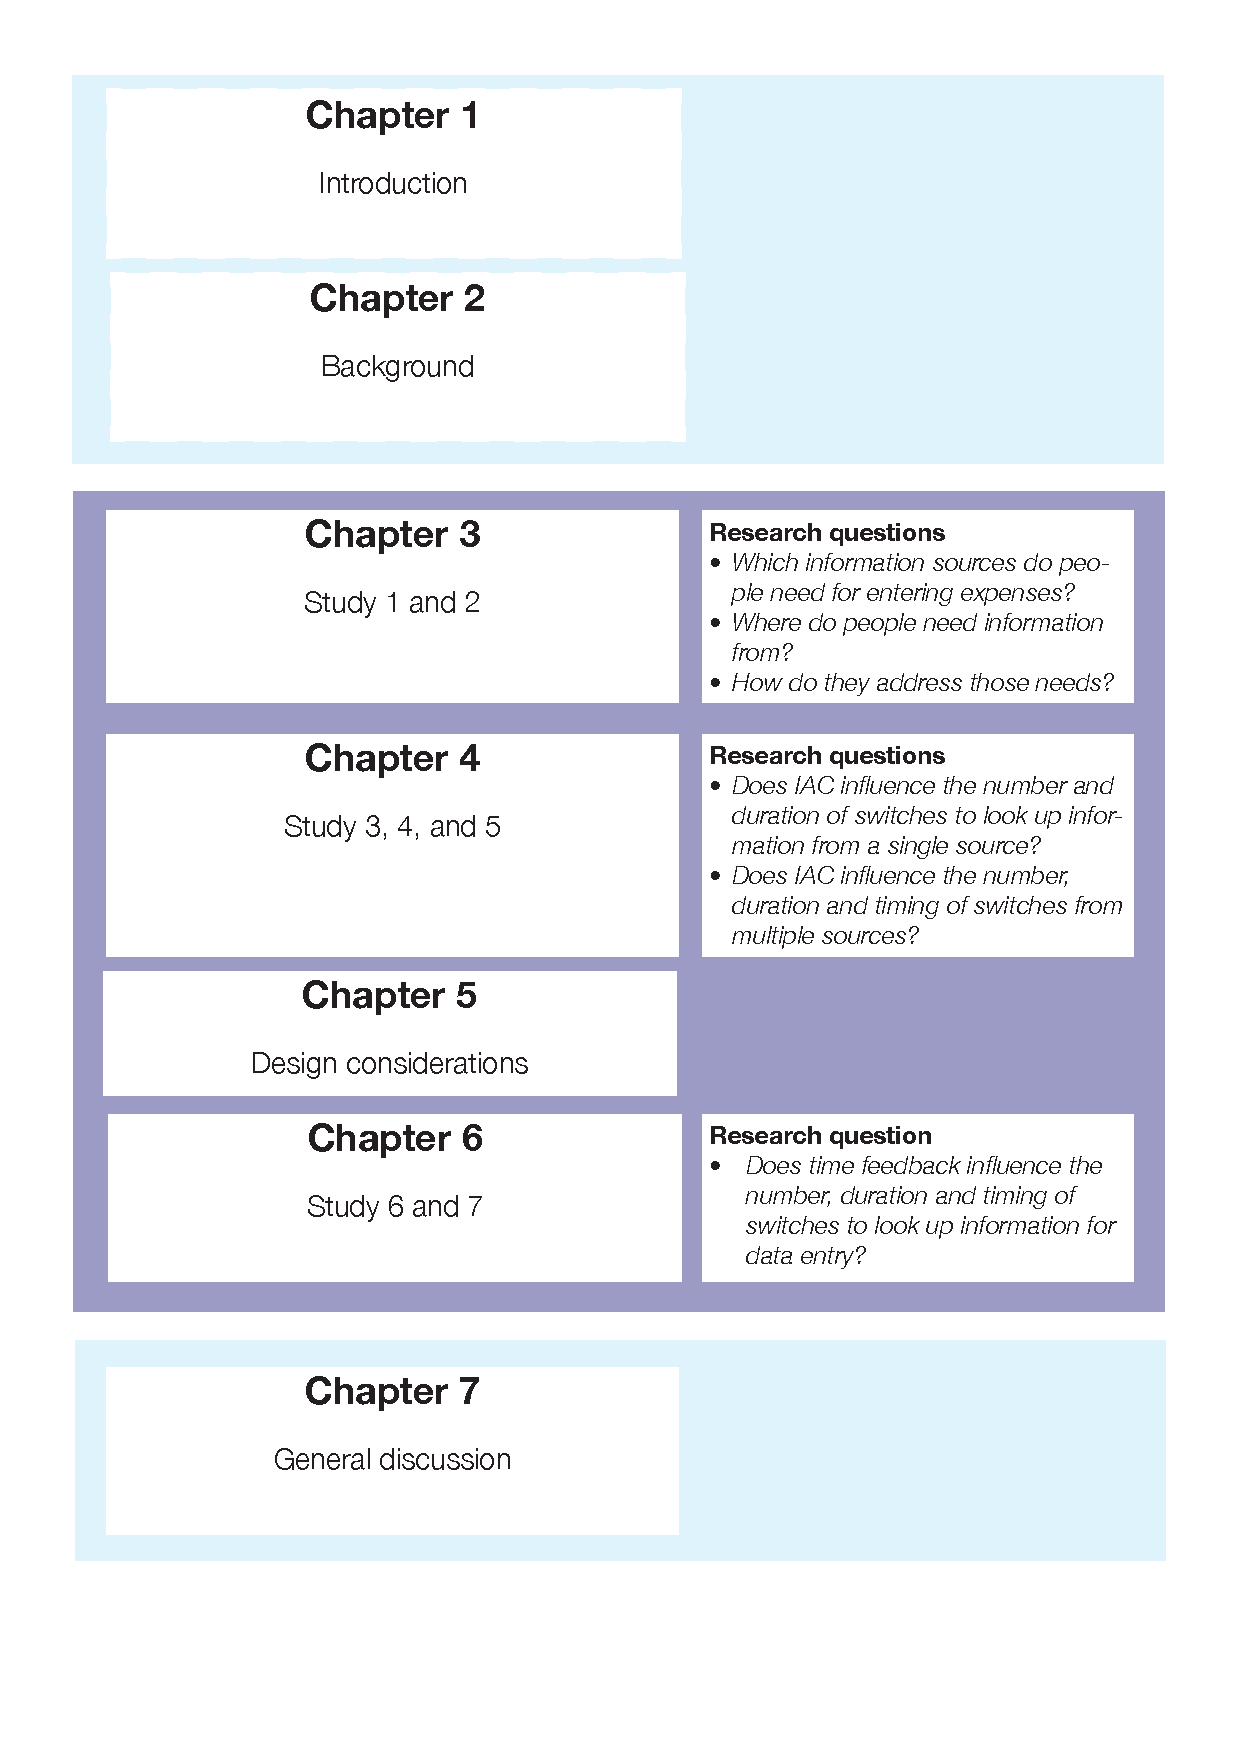
\includegraphics[width=0.7\textwidth]{images/ThesisOverview.pdf}
\caption{Visual overview of the thesis structure.}
%\vspace{-3pt}
\label{fig:ch1-thesisoverview}
\end{figure}

\pagebreak

\section{Contributions}
The thesis makes a number of contributions to HCI research. 

\textbf{C1 - Time costs affect self-interruption behaviour}

%Knowledge
The first contribution of my thesis is an increased understanding of the effect of time costs on people's self-interruption behaviour to collect task-related information. Prior work has shown that longer interruptions are more disruptive than short ones, but to date it was unclear how time costs affect people's decisions when and whether to address self-interruptions. My thesis demonstrates that the presumed time cost of an interruption determines whether an interruption is addressed straight away (if it is presumed to be short), or if it is postponed until a more convenient moment in the task (if it is presumed to be long). I also show that in a controlled environment, people are able to learn the time costs of digital interruptions and adapt their strategies to first address interruptions with a low time cost, before addressing interruptions with a high time cost. Outside of a controlled setting, these time costs are much harder to predict, and interruptions can end up taking much longer than expected or intended: users may have to go in and out of several computer windows, find the right information within information sources with task-irrelevant information, and get distracted. This means that people cannot always use expected time costs to effectively manage their interruptions. 

\textbf{C2 – Inquiries are handled differently than task-irrelevant self-interruptions}

The second contribution of the thesis is that it shows that inquiries are handled differently than task-irrelevant self-interruptions: whereas irrelevant interruptions may be ignored, depending on individual differences in ability to self-control interruptions \citep{Lyngs2018}, inquiries have to be addressed in order to progress with work. Contrary to the idea that focus on an activity can be improved by temporarily blocking distracting sources \citep{Kim2017}, my work shows that inquiries to distracting sources are considered part of the activity, and need different treatment. 

\textbf{C3 – Time feedback can help reduce time spent on interruptions}

%Design
These findings have implications for the design of any tools aiming to manage inquiries as well as other self-interruptions and distractions. A third, applied, contribution of this thesis is 
 is demonstrating how feedback on time spent on interruptions helps people reflect on actions during, and reduce the length of, their interruptions. Based on the understanding of how time costs affect self-interruption behaviour, a browser notification was developed and evaluated in this thesis. This browser notification showed people how long they are away from their data entry work, to make them more aware of time costs of their interruptions. %The information can make people reflect on what they are doing during prior interruptions, and it can encourage people to reduce the duration of subsequent interruptions.
%demonstrating how making time costs of interruptions visible can support people in managing these self-interruptions. 

\textbf{C4 – Data retrieval as a part of data entry research}

%By using the knowledge of the effect of time costs on people's self-interruption behaviour, a browser notification was developed and evaluated in this thesis. This design intervention 
%Methodology
Lastly, my work has implications for future data entry research. This thesis has highlighted that for some types of data entry work, a major component of the task is collecting data from various locations. Participants often spent a long time away from the data entry interface to find what they were looking for, which impacts how data is entered: it slows down data entry and increases likelihood of data entry errors. Data entry interfaces should take this into consideration and make it easier to resume a task. If data entry interfaces are intended to be used in situations where information is not readily available, they should be evaluated by requiring participants to first collect data from the environment, to determine how usable they are in this context. 

% Therefore, extending the theory that people always try to minimise time, my work shows that people are largely unaware of time. 
%inquiries are handled differently than other interruptions, and that time costs influence self-interruption behaviour. 

%The first contribution of this thesis is to map out the fragmented nature of an expenses task, of which looking up information is a substantial part of the task. It investigates how the time cost of accessing required information sources affects how people manage when they look up certain information. This finding has implications for the design of the current system: a second contribution is demonstrating how changing certain design features can better support people in managing these subtasks of looking up information.
